\documentclass[a4paper, 11pt, titlepage]{article}

% instead driver by specific driver name such as dvips  
%\usepackage[dvips]{graphicx}
\usepackage[dvips]{graphicx}
\usepackage{makeidx}
\usepackage{showidx}
\usepackage{verbatim}

\usepackage{lmodern}
\usepackage[T1]{fontenc}
\usepackage{textcomp}

\title{Second Day}
% add my email in the author name 
%\author{smher$<$\href{smhhaoo@126.com}{smher}$>$}    % can work !!!
%\author{smher $<$\href{mailto:smhhaoo@126.com}{smhhaoo@126.com}$>$}   % can work 
\author{\href{smhhaoo@126.com}{smher}}

\makeindex

\usepackage[xetex,colorlinks=true]{hyperref}    % caution the specific driver , see the 'texdoc hyperref' 
\hypersetup{colorlinks, %
			citecolor=black}       % Caution, the change of cite color !!!

% add the information of pdf file
\hypersetup{pdfauthor={smher}, %
			pdftitle={learn_tex}}

\begin{document}
\maketitle
%\frontmatter          % only for book, cannot used in book or report !!! ...
\tableofcontents
%\hypersetup{colorlinks=true}
\today

% U should know what is index mean firstly !!! ...
\printindex

\newpage
%\mainmatter
\part{FOUR}
\section{Professional func}
\subsection{Insert EPS pic.}

Firstly, showing a picture from a file:

\begin{figure}[!hbp]\label{pic1}
\centering
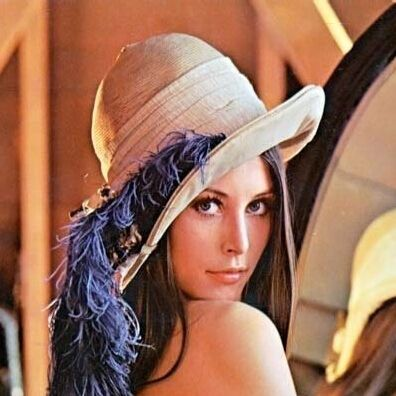
\includegraphics[angle=90,width=0.5\textwidth]{lena}
%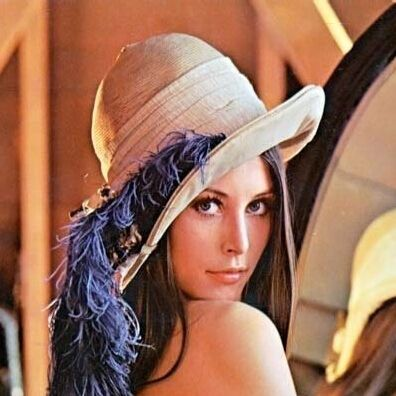
\includegraphics[angle=90,width=0.5\textwidth]{lena.jpg} % failed
\caption{This is a test.}
\end{figure}

As shown in pic.~\ref{pic1}, the insert picture operation is so easy. Paper~\cite{pa}, introduce the usage of \TeX{} very well. 

\index{pab} is show the \verb|\index| Usage. \\

This is the fundamental frame of C++ : \\
\verbatiminput{main.cpp}

\rightmark
\leftmark

\subsection{use pdf\LaTeX}
\subsubsection{publish online}
	use \verb|\pdfpagewidth = \paperwidth|
\begin{quote}
use \verb|\pdfpageheght=\paperheight|
\end{quote}
\subsubsection{font}
 best to use PostScript type 1.
\subsubsection{hyperef}
Go to Baidu, use this hype link:\\
\href{www.baidu.com}{Baidu} website.\\
link to a local file:\\
\href{main.cpp}{here}\\

\subsubsection{\texorpdfstring{$E=mc^2$}{E=mc^2}}
if the title include the unshown chars like math equation, use \verb|\texorpdfstring{text}{PDFstring}|

\newpage
\appendix
\section{References}
\begin{thebibliography}{99}
\bibitem{pa} H.~Partl:
\emph{German \TeX}, TUGboat Volumn~9, Issue~1(1998)
\bibitem{pb} SMH:
\emph{\TeX{} Usage} are working on ...
\end{thebibliography}

\index{pab} this is pab.\\
\index{pac} this is pac.

%\backmatter



\end{document}